% !TEX encoding = UTF-8 Unicode
%%%%%%%%%%%%%%%%%%%%%%%%%%%%%%%%%%%%%%%%%
% Beamer Presentation
% LaTeX Template
% Version 1.0 (10/11/12)
%
% This template has been downloaded from:
% http://www.LaTeXTemplates.com
%
% License:
% CC BY-NC-SA 3.0 (http://creativecommons.org/licenses/by-nc-sa/3.0/)
%
%%%%%%%%%%%%%%%%%%%%%%%%%%%%%%%%%%%%%%%%%

%----------------------------------------------------------------------------------------
%	PACKAGES AND THEMES
%----------------------------------------------------------------------------------------

\documentclass{beamer}

\mode<presentation> {

% The Beamer class comes with a number of default slide themes
% which change the colors and layouts of slides. Below this is a list
% of all the themes, uncomment each in turn to see what they look like.

%\usetheme{default}
%\usetheme{AnnArbor}
%\usetheme{Antibes}
%\usetheme{Bergen}
%\usetheme{Berkeley}
%\usetheme{Berlin}
%\usetheme{Boadilla}
%\usetheme{CambridgeUS}
%\usetheme{Copenhagen}
%\usetheme{Darmstadt}
%\usetheme{Dresden}
%\usetheme{Frankfurt}
%\usetheme{Goettingen}
%\usetheme{Hannover}
%\usetheme{Ilmenau}
%\usetheme{JuanLesPins}
%\usetheme{Luebeck}
\usetheme{Madrid}
%\usetheme{Malmoe}
%\usetheme{Marburg}
%\usetheme{Montpellier}
%\usetheme{PaloAlto}
%\usetheme{Pittsburgh}
%\usetheme{Rochester}
%\usetheme{Singapore}
%\usetheme{Szeged}
%\usetheme{Warsaw}

% As well as themes, the Beamer class has a number of color themes
% for any slide theme. Uncomment each of these in turn to see how it
% changes the colors of your current slide theme.

%\usecolortheme{albatross}
%\usecolortheme{beaver}
%\usecolortheme{beetle}
%\usecolortheme{crane}
%\usecolortheme{dolphin}
%\usecolortheme{dove}
%\usecolortheme{fly}
%\usecolortheme{lily}
%\usecolortheme{orchid}
%\usecolortheme{rose}
%\usecolortheme{seagull}
%\usecolortheme{seahorse}
%\usecolortheme{whale}
%\usecolortheme{wolverine}

%\setbeamertemplate{footline} % To remove the footer line in all slides uncomment this line
%\setbeamertemplate{footline}[page number] % To replace the footer line in all slides with a simple slide count uncomment this line

%\setbeamertemplate{navigation symbols}{} % To remove the navigation symbols from the bottom of all slides uncomment this line
}

\usepackage{graphicx} % Allows including images
\usepackage{booktabs} % Allows the use of \toprule, \midrule and \bottomrule in tables
\usepackage{xeCJK}
\usepackage{color}
\usepackage{listings}

%----------------------------------------------------------------------------------------
%	TITLE PAGE
%----------------------------------------------------------------------------------------

\title[Linux System Programming]{Linux System Programming} % The short title appears at the bottom of every slide, the full title is only on the title page

\author{张海宁} % Your name
\institute[贵大计算机] % Your institution as it will appear on the bottom of every slide, may be shorthand to save space
{
贵州大学 \\ % Your institution for the title page
\medskip
\textit{hnzhang1@gzu.edu.cn} % Your email address
}
\date{\today} % Date, can be changed to a custom date

\begin{document}

\begin{frame}
\titlepage % Print the title page as the first slide
\end{frame}

\begin{frame}
\frametitle{Overview} % Table of contents slide, comment this block out to remove it
\tableofcontents % Throughout your presentation, if you choose to use \section{} and \subsection{} commands, these will automatically be printed on this slide as an overview of your presentation
\end{frame}

%----------------------------------------------------------------------------------------
%	PRESENTATION SLIDES
%----------------------------------------------------------------------------------------

%------------------------------------------------
\section{System Programming} % Sections can be created in order to organize your presentation into discrete blocks, all sections and subsections are automatically printed in the table of contents as an overview of the talk
%------------------------------------------------
\begin{frame}
\frametitle{System Programming}
System programming is the art of writing system software.System software lives at a low level, interfacing directly with the \textcolor{red}{kernel and core system libraries}.

There are three cornerstones to system programming in Linux: 
\begin{enumerate}
\item system calls
\item the C library
\item the C compiler
\end{enumerate} 
\end{frame}
%\subsection{System Calls} % A subsection can be created just before a set of slides with a common theme to further break down your presentation into chunks

\begin{frame}
\frametitle{System Calls}
System programming starts with system calls.System calls (often shorted to syscalls) are \textcolor{red}{function invocations} made from \textcolor{red}{user space}—your text editor, favorite game, and so on—\textcolor{red}{into the kernel} (the core internals of the system) in order to request some service or resource from the operating system. 
\end{frame}
\begin{frame}
\frametitle{Invoke system calls}
It is not possible to directly link user-space applications with kernel space. For reasons of security and reliability, user-space applications must not be allowed to directly execute kernel code or manipulate kernel data. Instead, the kernel must provide a mechanism by which a user-space application can "signal" the kernel that it wishes to invoke a system call. The application can then trap into the kernel through this well-defined mechanism, and execute only code that the kernel allows it to execute. The exact mechanism varies from architecture to architecture.
\end{frame}


%------------------------------------------------
\begin{frame}
\frametitle{The C Library}
The C library (\textcolor{red}{libc}) is at the heart of Unix applications. Even when you're programming in another language, the C library is most likely in play, wrapped by the higher-level libraries, providing core services, and facilitating system call invocation. On modern Linux systems, the C library is provided by GNU libc, abbreviated \textcolor{red}{glibc}, and pronounced gee-lib-see or, less commonly, glib-see.

The GNU C library provides more than its name suggests. In addition to implementing the standard C library, glibc provides wrappers for system calls, threading support, and basic application facilities.
\end{frame}

%-------------------------------------------------
\begin{frame}
\frametitle{The C Compiler}
In Linux, the standard C compiler is provided by the \textcolor{red}{GNU Compiler Collection (gcc)}. Originally, gcc was GNU's version of cc, the C Compiler. Thus, gcc stood for \textcolor{red}{GNU C Compiler}. Over time, support was added for more and more languages. Consequently, nowadays gcc is used as the generic name for the family of GNU compilers. However, gcc is also the binary used to invoke the C compiler. In this course, when we talk of gcc, we typically mean the program gcc, unless context suggests otherwise.

\end{frame}

%------------------------------------------------

\begin{frame}
\frametitle{用户程序vs库函数vs系统调用}

\begin{figure}
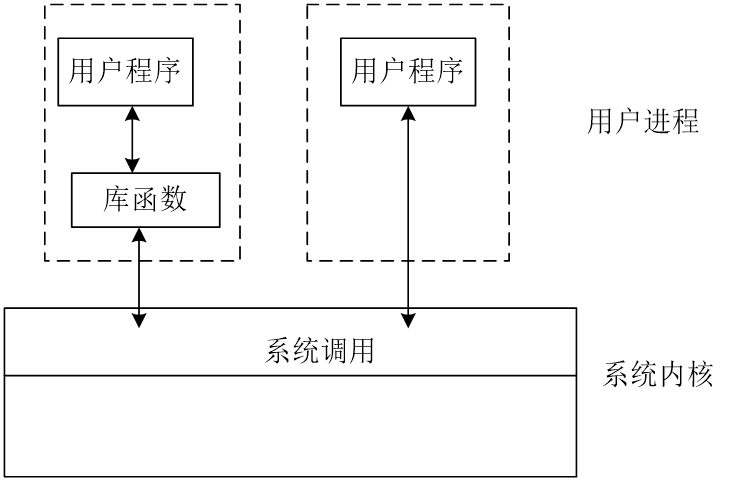
\includegraphics[width=1\linewidth]{601}
\end{figure}
\end{frame}
%------------------------------------------------
\section{GCC}
\begin{frame}
\frametitle{GCC}
The \textcolor{red}{GNU Compiler Collection} includes front ends for C, C++, Objective-C, Fortran, Ada, and Go, as well as libraries for these languages (libstdc++,...). GCC was originally written as the compiler for the GNU operating system. 

The GNU system was developed to be 100\% free software, free in the sense that it respects the \textcolor{red}{user's freedom}.

\end{frame}
\begin{frame}
\frametitle{The four essential freedoms}
A program is free software if the program's users have the four essential freedoms:
\begin{itemize}
\item
The freedom to \textcolor{red}{run} the program as you wish, for any purpose (freedom 0).
\item
The freedom to \textcolor{red}{study} how the program works, and \textcolor{red}{change} it so it does your computing as you wish (freedom 1). Access to the source code is a precondition for this.
\item
The freedom to \textcolor{red}{redistribute} copies so you can help others (freedom 2).
\item
The freedom to \textcolor{red}{distribute copies of your modified versions} to others (freedom 3). By doing this you can give the whole community a chance to benefit from your changes. Access to the source code is a precondition for this.
\end{itemize}
\url{https://www.gnu.org/philosophy/free-sw.html}

\end{frame}
%---------------------------------------------
\begin{frame}
\frametitle{GNU Toolchain}
GCC is a key component of "GNU Toolchain", for developing applications, as well as operating systems. The GNU Toolchain includes:
\begin{itemize}
\item GNU Compiler Collection (GCC): a compiler suit that supports many languages, such as C/C++ and Objective-C/C++
\item GNU Make: an automation tool for compiling and building applications
\item GNU Binutils: a suit of binary utility tools, including linker and assembler
\item GNU Debugger (GDB)
\item GNU Autotools: A build system including Autoconf, Autoheader, Automake and Libtool
\item GNU Bison: a parser generator (similar to lex and yacc)
\end{itemize}
\end{frame}
\begin{frame}
\frametitle{Platform}
GCC is portable and run in many operating platforms.

 GCC (and GNU Toolchain) is currently available on all \textcolor{red}{Unixes}. They are also ported to \textcolor{red}{Windows} (by MinGW and Cygwin). GCC is also a cross-compiler, for producing executables on different platform.
\end{frame}
\begin{frame}
\frametitle{Install gcc}
\begin{itemize}
\item Unix/Linux/Mac GCC(GNU Toolchain) is included.
\item Windows
\begin{itemize}
\item Cygwin GCC: Cygwin is a Unix-like environment and command-line interface for Microsoft Windows. Cygwin is huge and includes most of the Unix tools and utilities. It also included the commonly-used Bash shell.
\item MinGW: MinGW (Minimalist GNU for Windows) is a port of the GNU Compiler Collection (GCC) and GNU Binutils for use in Windows. It also included MSYS (Minimal System), which is basically a Bourne shell (bash).
\end{itemize}
\end{itemize}
\end{frame}

\begin{frame}[fragile]
\frametitle{Versions and Help}
We can display the version of GCC with --version/-v option, and get help with --help option:
\begin{example}[show version and help of GCC]
\begin{verbatim}
$ gcc -v
$ gcc --version
$ gcc --help
\end{verbatim}
\end{example}
\end{frame}

\subsection{Using GCC}
\begin{frame}
\frametitle{编写c程序的流程}
\begin{figure}
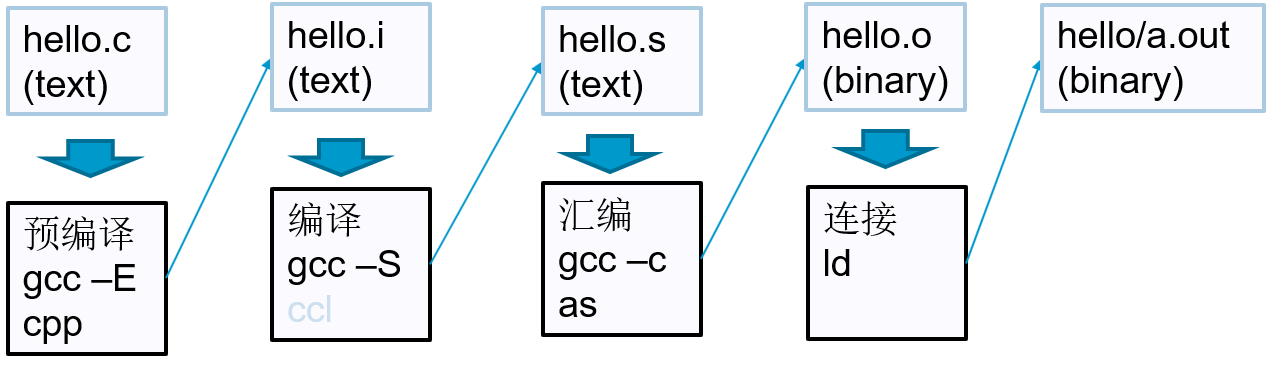
\includegraphics[width=1\linewidth]{602}
\end{figure}
\end{frame}
\begin{frame}
\frametitle{编写c程序的流程}
\begin{figure}
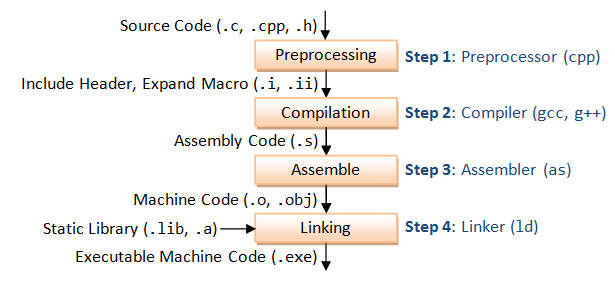
\includegraphics[width=1\linewidth]{603}
\end{figure}
\end{frame}

\begin{frame}[fragile]
\frametitle{hello.c}
\begin{example}
\begin{verbatim}
// hello.c
#include <stdio.h>

int main(){
        printf("Hello, C.\n");
        return 0;
}
\end{verbatim}
\end{example}
\end{frame}



%------------------------------------------
\begin{frame}
\frametitle{从.c文件到可执行文件}
\begin{block}{预处理}
gcc -E hello.c -o hello.i
\end{block}

\begin{block}{编译}
gcc -S hello.i
hello.s
\end{block}

\begin{block}{汇编}
gcc -c hello.s -o hello.o
hello.o
\end{block}
\begin{block}{链接}
gcc hello.o -o hello.out
\end{block}

\begin{block}{all in one}
gcc hello.c -o hello.out
\end{block}
\end{frame}

%-------------------------------------------------
\subsection{库文件}
\begin{frame}
\frametitle{静态库和动态库}
库文件是一组补预先编译的目标文件的集合,可以被链接到用户所编写的程序中。
\begin{itemize}
\item 静态库

通常以“.a”结尾(archive file),静态库的代码在编译时就会连接到用户的程序中
\item 动态库

通常以“.so”结尾(shared objects),用户的程序在运行时,按需要载入
\end{itemize}

\end{frame}
\subsection{补充工具}
\begin{frame}
\frametitle{几个有用的工具}
\begin{enumerate}
\item file

判断文件的类型
\item nm

显示目标文件的符号表,通常用于查看目标文件中是否定义了某个特定的函数

\item ldd

检查一个可执行文件并显示出其需要的动态库文件

\item
mtrace

内存溢出检测

\end{enumerate}
\end{frame}
%-----------------------------------------------
\section{make}
\begin{frame}
\frametitle{make}
依照makefile文件,make程序可以自动确定一个软件包的哪些部分需要重新编译。

makefile文件描述了建立可执行程序的一些规则。
\end{frame}
%------------------------------------------------

\begin{frame}[fragile]
\frametitle{makefile}
\begin{columns}[c] % The "c" option specifies centered vertical alignment while the "t" option is used for top vertical alignment

\column{.45\textwidth} % Left column and width
\textbf{hello.c}
\lstset{language=C}
\begin{lstlisting}

// hello.c
#include <stdio.h>

int main(){
    printf("Hello,C.\n");
    return 0;
}

\end{lstlisting}
\column{.5\textwidth} % Right column and width
\textbf{makefile}
\begin{lstlisting}
all:hello

hello:hello.o
        gcc -o hello hello.o

hello.o:hello.c
        gcc -c hello.c
clean:
        rm hello.o
\end{lstlisting}

\end{columns}
\end{frame}
\begin{frame}[fragile]
\frametitle{makefile的规则}
\begin{lstlisting}
target: pre-req-1 pre-req-2 ...
	command
\end{lstlisting}
The target and pre-requisites are separated by a colon (:). The command must be preceded by a tab (NOT spaces).
\end{frame}
\begin{frame}[fragile]
\frametitle{make和makefile}
\begin{lstlisting}
$ make
gcc -c hello.c
gcc -o hello hello.o
$ make clean
rm hello.o
$ ls
hello  hello.c  makefile
\end{lstlisting}
\end{frame}

\begin{frame}[fragile]
\frametitle{修改源文件与make的关系}
\begin{lstlisting}
$ make
gcc -c hello.c
gcc -o hello hello.o
$ make
make: Nothing to be done for 'all'.
$ vim hello.c
$ make
gcc -c hello.c
gcc -o hello hello.o
$ ./hello
Hello, C.
test make.
\end{lstlisting}
\end{frame}
%------------------------------------------------
\section{GDB}
%------------------------------------------------
\begin{frame}
\frametitle{GDB}
GDB(GNU Source-Level Debugger),是GNU的一个\textcolor{red}{命令行调试工具}。它主要可以完成以下功能:
\begin{itemize}
\item
设置运行环境和参数运行指定程序
\item
让程序在指定的条件下停止
\item
当程序停止时,检查发生了什么
\item
改变正在调试的程序,以修正某个bug,然后继续调试
\end{itemize}
\end{frame}
\begin{frame}
\frametitle{gdb部分命令}
\begin{table}
\begin{tabular}{l l l l }
\toprule
\textbf{命令} & \textbf{作用} & \textbf{命令} & \textbf{作用}\\
\midrule
file & 载入可执行文件 & list & 显示源代码 \\
run & 执行 & info local & 显示当前函数中变量值 \\
kill & 停止执行 & info break & 显示断点列表 \\
break & 设置断点 & info func & 显示所有函数名 \\
delete & 删除断点 & watch & 监视表达式的变化 \\
print & 显示表达式的值 & next & 执行下一条代码,但不进入 \\
shell命令 & 执行shell命令 & step & 执行下一条代码,进入函数 \\
\bottomrule
\end{tabular}
\caption{GDB部分命令}
\end{table}
\end{frame}

\begin{frame}[fragile]
\frametitle{gdb示例}
\begin{lstlisting}
$ vim gdb.c
$ cat gdb.c
#include <stdio.h>
int main(){
        int i=0;
        for(i=0;i<=15;i++){
                printf("the number is %d",i);
        }
}
$ gcc -ggdb -o gdbTest gdb.c
\end{lstlisting}
\end{frame}

\begin{frame}
\frametitle{gdb示例}
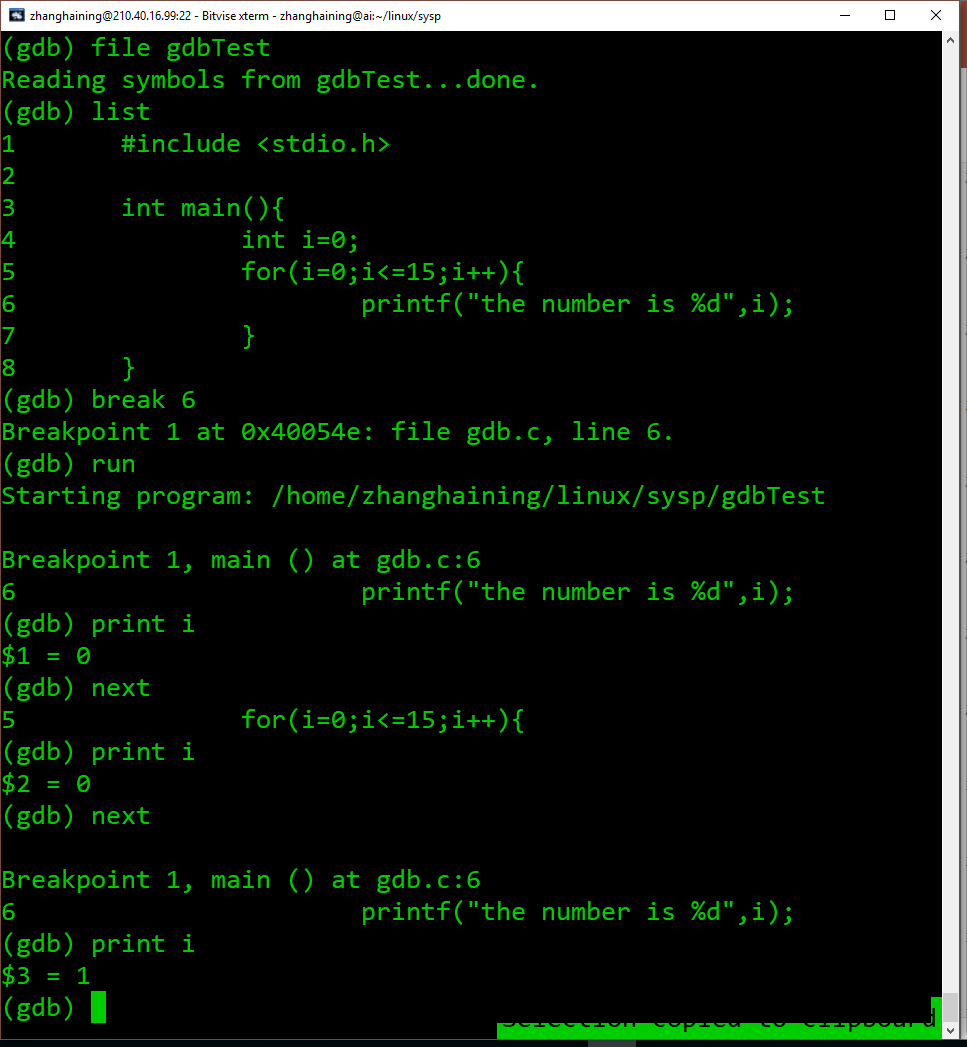
\includegraphics[width=0.8\linewidth]{605}

\end{frame}
%------------------------------------------------
\begin{frame}
\Huge{\centerline{总结}}
\begin{enumerate}
\item
System Call,C Compiler,C Library
\item
GCC
\item
make,makefile
\item
GDB
\end{enumerate}

\end{frame}

%------------------------------------------------
\begin{frame}
\frametitle{作业}
按以下要求进行编程练习:
\begin{enumerate}
\item
2个cpp文件:prog.cpp, aux.cpp
\item
1个h文件:aux.h
\item
aux.h头文件定义函数Max和Min,它们分别计算四个数(参数)的最大值和最小值;aux.cpp实现这两个函数
\item
prog.c中定义主函数,循环输入4个随机数,输出他们的最大和最小值
\item
编译该项目,调试、跟踪程序执行过程;并在控制台界面运行编译的可执行文件。
\item
\textcolor{red}{编写类似功能的c语言程序也可。}
\end{enumerate}
\end{frame}


%------------------------------------------------

\begin{frame}
\Huge{\centerline{The End}}
\end{frame}

%----------------------------------------------------------------------------------------

\end{document} 